\documentclass[14pt,a4paper]{scrartcl}
\usepackage[english,russian]{babel}
\usepackage[T2A]{fontenc}
\usepackage{setspace}
\usepackage[left=5mm,right=5mm, top=3mm,bottom=3mm,bindingoffset=0cm]{geometry}
\usepackage{graphicx}
\usepackage{multicol}
\usepackage{amsmath}
\usepackage{amssymb}
\usepackage{array}

\pagenumbering{gobble}

\begin{document}

	\columnsep=30pt
	\begin{multicols}{2}

		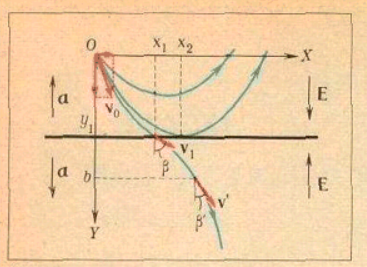
\includegraphics{Picture.PNG}

		{\small Рис. 2.}	
		\vspace{3mm}

		одна "--- выше плоскости, а~другая "--- ниже. 
		Роль ускорения свободного падения $g$ играет ускорения $a$.
		Для~того~чтобы ответить на~другие вопросы задачи, нужно рассмотреть два случая: а)~пластина заряжена отрицательно и~б)~пластина заряжена положительно.

		Рассмотрим случай~а). 
		В~этом случае вектор напряженности электрического поля направлен к~пластинке, а~ускорение $a$ электрона "--- от~пластины. 
		Несколько возможных траекторий движения электрона (для~разных значений $\sigma$) показаны на~рисунке~2. 
		Если~ускорение <<свободного падения>> $a$ велико, то~электрон может~и~ не~достигнуть пластины. 
		Так~как~вертикальная составляющая начальной скорости электрона равна $\upsilon_y=\upsilon_0\cos \alpha$, то~максимальная высота $H$ его <<подъема>> равна
		\[
			H=\frac{\upsilon_y^2}{2a}=\frac{(\upsilon_0\cos \alpha)^2}{2a}=
\frac{(\upsilon_0 \cos \alpha)^2 \varepsilon_0 m}{\varepsilon \sigma}. \tag{3} \label{3}
		\]

		Если $H<d$, то~это значит, что~электрон не~долетит до~пластины. В~этом случае минимальное расстояние, на~которое электрон приблизится к~пластине, равно
		\[
			h=d-H=d-\frac{(\upsilon_0 \cos \alpha)^2 \varepsilon_0 m}{\varepsilon \sigma}.		
		\]

		При~$H=d$ траектория электрона касается пластины, а~при~$H>d$ электрон пролетит пластину. Ниже пластины траекторией движения электрона будет другая парабола.
		И~так~как здесь ускорение направлено от~пластины, то~электрон будет все время удаляться от~нее.
		
		Найдем, в~какой точке электрон пролетит через~пластину и~скорось его в~этот момент времени. 
		Для~этого запишем уравнения движения электрона. 
		Проекция скорости электрона на~ось $X$ (рис.~2) постоянна и~равна~$\upsilon_x=\upsilon_0 \sin \alpha$. Поэтому координата $x$ электрона меняется со~временем по~закону
		\[
			x=\upsilon_x t = \upsilon_0 \sin \alpha \cdot t. \tag{4} \label{4}
		\]

		Так~как~ускорение электрона $a$ направлено вдоль оси~$Y$, то~координата $y$ меняется со~временем~так:
		\[
			y=\upsilon_0 \cos \alpha \cdot t + \frac{a t^2}{2}. \tag{5} \label{5}
		\]

		В~момент времени $t=t_1$, в~который электрон пересекает пластину, $y=y_1=d$ и~$x=x_1$. Подставив эти значения $t$, $x$ и~$y$ в~уравнения \eqref{4} и~\eqref{5}, получим:
		\[
			x_1=\upsilon_0 \sin \alpha \cdot t_1{,}
		\]
		\[
			d=\upsilon_0 \cos \alpha \cdot t_1 + \frac{a t^2_1}{2}. \tag{6} \label{6}
		\]
		Решая эту~систему уравнений, найдем
		\[
			t_1=\frac{- \upsilon_0 \cos \alpha + \sqrt{\upsilon_0^2 \cos^2 \alpha + 2ad}\ }{a}^*\Biggr), \tag{7} \label{7}
		\]
		\[
			x_1=\upsilon_0 \sin \alpha \cdot \frac{- \upsilon_0 \cos \alpha + \sqrt{\upsilon_0^2 \cos^2 \alpha + 2ad}}{a}
		\]

		\vspace{1mm}
		\noindent\rule{\textwidth}{0,5pt}
		\vspace{1mm}
		
		{\small *) Решая второе из~уравнений (6), мы отбросили второй, больший корень $t_1$. Это~уравнение позволит определить те~моменты времени, когда частица имеля координату $y$, равную $d$. Если~бы~пластина находилась далеко и~электрон не~пересекал~бы ее~при~своем движении, то~это~значение $y$ повторялось~бы дважды: первый~раз, когда электрон <<поднимался>>, и~второй~раз, когда "--- <<падал>>. Значению координаты $y=d$ при~<<возвращении>> электрона и~соответствует второй корень $t_1$, равный
		\[
			\frac{- \upsilon_0 \cos \alpha - \sqrt{\upsilon_0^2 \cos^2 \alpha + 2ad}}{a}
		\]}

	\end{multicols}
	
	\begin{flushleft}
		{\small \textbf{36}}
	\end{flushleft}

\end{document}